\section{wxPython}


\begin{frame}{Grafische Benutzeroberfl"achen (GUIs)}
%% 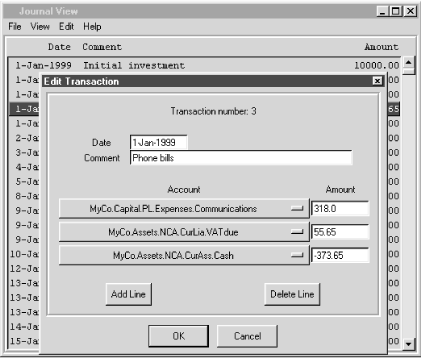
\includegraphics[height=4.3cm]{images/tkinter.png}
%% \hspace*{2mm}
%% 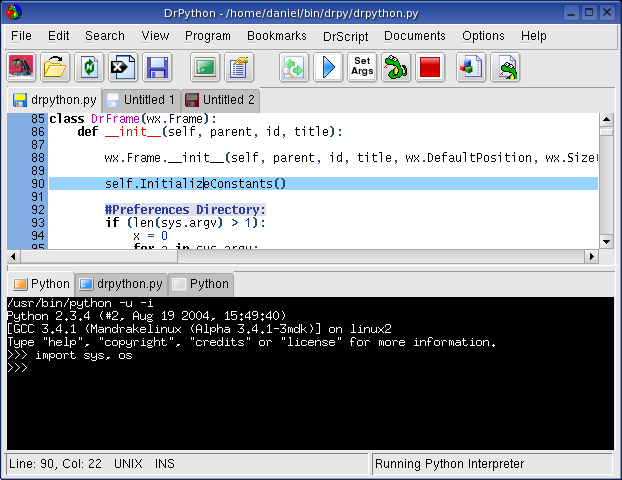
\includegraphics[height=4.3cm]{images/drpython_screenshot.png}

Verbreitete GUI-Toolkits mit Bindings f"ur (u.A.) Python:
\begin{itemize}
\item \alert{Tk}: In Python's Standardbibliothek, simpel (ungeeignet f"ur komplexe Anwendungen), veraltetes Aussehen
\item \alert{GTK}: z.B. Gnome Desktop, GIMP, Eclipse, \dots
\item \alert{QT}: KDE Desktop, Skype, Scribus, \dots
\end{itemize}
Alle werden auf den g"angingen Betriebssystemen unterst"utzt.
\vspace{3mm}
\begin{itemize}
\item \alert{wxWidgets}: Benutzt  Windows-, Mac OS-Bibliotheken oder GTK $\rightarrow$~Look and Feel des jeweiligen Betriebssystems
\end{itemize}
\end{frame}

\begin{frame}{Die wxPython-Demo}
\lstinline{/usr/share/doc/wx2.8-examples/examples/wxPython/demo.py}\\[2mm]
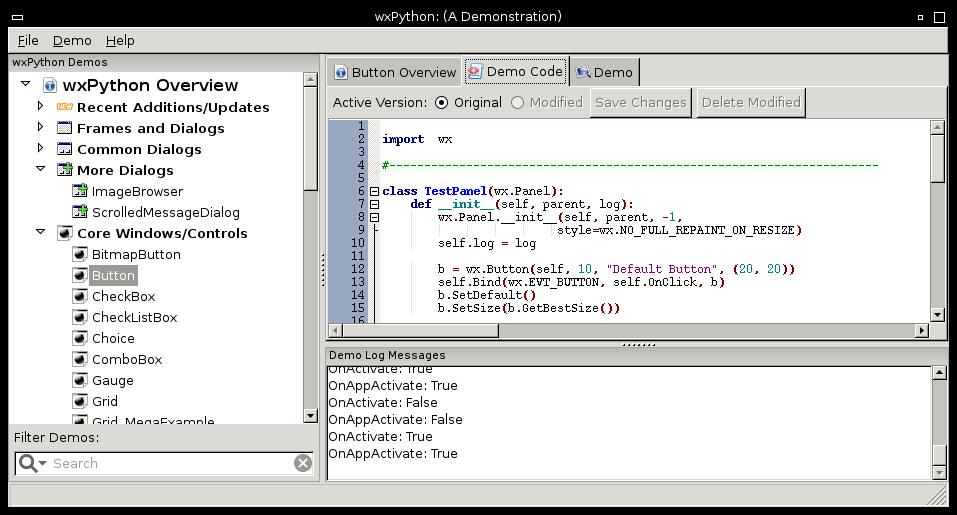
\includegraphics[width=\textwidth]{images/wxpython_demo.png}\\
Kurze Beschreibung aller Features mit Live-Demo und Beispiel-Code
\end{frame}

\begin{frame}[fragile]{Hello World}
\begin{lstlisting}[style=Python]
import wx

class MainFrame(wx.Frame):
   def __init__(self):
      wx.Frame.__init__(self, parent=None, 
                        title="Hello World")
      self.Show(True)

app = wx.PySimpleApp()
frame = MainFrame()
app.MainLoop()
\end{lstlisting}
Erzeugt ein leeres Fenster mit Titel \glqq Hello World\grqq.
\end{frame}

\begin{frame}{Die Basis: Application und Top Level Windows}
\alert{Application:}
\begin{itemize}
\item Kern eines wx-Programms, betreibt die \alert{Hauptschleife}
\item Hauptschleife verarbeitet alle \alert{Events} (Mausbewegung, Tastaturanschlag, \dots)
\item \lstinline{PySimpleApp}: F"ur einfache Anwendungen mit nur einem Top Level Window
\end{itemize}
\vspace{3mm}
Zur Application geh"ort mindestens ein \alert{Top Level Window}:
\begin{itemize}
\item Pr"asentiert dem Anwender die wichtigsten Datan und Kontrollelemente
\item Wird das letzte Top Level Window geschlossen, beendet sich die Application (die Hauptschleife wird verlassen)
\end{itemize}
\end{frame}

\begin{frame}[fragile]{Das allgemeinste Widget: wx.Frame}
\begin{lstlisting}[style=Python]
wx.Frame(parent, id=-1, title="", 
         pos=(-1,-1), size=(-1,-1), ...)
\end{lstlisting}
\begin{itemize}
\item \alert{parent}: Ist \lstinline{None} f"ur Top Level Windows
\item \alert{id}: Integer; Automatische Generierung mit -1 (zu bevorzugen) 
\item \alert{title}: Fenstertitel, wird in Titelleiste angezeigt
\item \alert{pos}: Integer-Tupel (x, y); (-1, -1) l"asst das unterliegende System entscheiden
\item \alert{size}: Integer-Tupel (width, height); (-1, -1) l"asst das unterliegende System entscheiden
\end{itemize}
\end{frame}

\begin{frame}[fragile]{Widgets in ein Frame einf"ugen}
Etwas Text in unserem Fenster:
\begin{lstlisting}[style=Python]
class MainFrame(wx.Frame):
   def __init__(self):
      wx.Frame.__init__(self, parent=None, 
                        title="Hello World")
      panel = wx.Panel(parent=self)
      wx.StaticText(parent=panel,
                    label="How are you?")
      self.Show(True)
\end{lstlisting}
\end{frame}

\begin{frame}[fragile]{Widgets in ein Frame einf"ugen}
\begin{columns}
\begin{column}{0.35\textwidth}
\begin{tikzpicture}
  \shadedraw [top color=plightgrey, bottom color=plightgrey] (0,0) rectangle (4,-6);
  \draw (0,0) node [anchor=north west]{wx.Frame};
  \shadedraw [top color=white, bottom color=white] (0.3,-1) rectangle (3.7,-5.7);
  \draw (0.3,-1) node [anchor=north west]{wx.Panel};
  \draw (0.6,-2.2) node [anchor=west, draw, fill=plightyellow] {wx.StaticText};
  \draw (0.6,-3.2) node [anchor=west, draw, fill=plightyellow] {wx.StaticText};
  \draw (0.6,-4.2) node [anchor=west, draw, fill=plightyellow] {wx. ...};
\end{tikzpicture}
\end{column}

\begin{column}{0.65\textwidth}
\begin{itemize}
\item \alert{Panel}: Container, welcher beliebig viele weitere Widgets enthalten kann.
\item Parent-Beziehungen legen fest, welches Widget in welchem Widget dargestellt wird
\end{itemize}
\end{column}
\end{columns}
\end{frame}

\begin{frame}[fragile]{Nicht-editierbarer Text: StaticText}
\begin{lstlisting}[style=Python]
wx.StaticText(parent, id=-1, label="", 
              pos=(-1,-1), size=(-1,-1), 
              style=0, ...)
\end{lstlisting}
\begin{itemize}
\item \alert{label}: Der darzustellende Text
\item \alert{pos} bezieht sich auf die Position innerhalb des Parent-Widgets
\item \alert{style}: \lstinline{wx.ALIGN_CENTER}, \lstinline{wx.ALIGN_LEFT}, \lstinline{wx.ALIGN_RIGHT}
\item Auch mehrzeiliger Text m"oglich
\item Einige Methoden:
\begin{itemize}
\item \lstinline{SetLabel}: Text nachtr"aglich "andern
\item \lstinline{SetForegroundColour}, \lstinline{SetBackgroundColour}
\item \lstinline{SetFont}
\end{itemize}
\end{itemize}
\end{frame}

\begin{frame}[fragile]{Auf Benutzeraktionen reagieren}
\begin{lstlisting}[style=Python]
class MainFrame(wx.Frame):
   def __init__(self):
      wx.Frame.__init__(parent=None)
      panel = wx.Panel(parent=self)
      button = wx.Button(parent=panel,
                         label="&Click me")
      self.Bind(wx.EVT_BUTTON, self.on_button,
                button)
      self.Show(True)

   def on_button(self, evt):
      print "You pressed the button!"
\end{lstlisting}
Der Button kann mit Alt+C \glqq geclickt\grqq{} werden (wg. \lstinline{&C...})
\end{frame}

\begin{frame}[fragile]{Ereignisgesteuerte Programmierung}
\begin{itemize}
\item Herk"ommliche Programme laufen linear ab
\item GUI-Programme: Anwender kann Bedienelemente zu beliebiger Zeit in beliebiger Reihenfolge bedienen
\item GUI-Programm \emph{reagiert} auf den Anwender
\item $\rightarrow$ \alert{Hauptschleife} wartet auf \alert{Events} und leitet diese an passende \alert{Event-Handler} weiter
\end{itemize}
%\vspace{3mm}
\begin{lstlisting}[style=Python]
self.Bind(wx.EVT_BUTTON, self.on_button, 
          button)
\end{lstlisting}
\lstinline{MainFrame} soll alle Button-Events vom Widget {\lstinline{button}} mit der Methode \lstinline{onButton} behandeln.
\end{frame}

\begin{frame}[fragile]{Events und die Widget-Hierarchie}
\begin{lstlisting}[style=Python]
class MainFrame(wx.Frame):
   def __init__(self):
      ...
      self.Bind(wx.EVT_BUTTON,
                self.on_buttonF, button)
      button.Bind(wx.EVT_BUTTON,
                  self.on_buttonB, button)

   def on_buttonF(self, evt):
      print "You pressed the button!"

   def on_buttonB(self, evt):
      print "You pressed me!"
\end{lstlisting}
\end{frame}

\begin{frame}[fragile]{Events und die Widget-Hierarchie}
\begin{itemize}
\item Widget generiert Event
\item Hat das Widget passenden Event-Handler?
  \begin{itemize} 
    \item{ja}: behandle Event
    \item{nein}: Sende Event an das Parent-Widget
  \end{itemize}
\item Hat das Parent-Event passenden Event-Handler? \dots
\end{itemize}
$\rightarrow$ Nur \lstinline{onButtonB} wird ausgef"uhrt!\\[3mm]

Behandeltes Event wird weiter propagieren mit \alert{Skip}:
\begin{lstlisting}[style=Python]
def on_buttonB(self, evt):
   print "You pressed me!"
   evt.Skip()
\end{lstlisting}
$\rightarrow$ \lstinline{onButtonB} und \lstinline{onButtonF} werden ausgef"uhrt
\end{frame}

\begin{frame}{Widgets anordnen mit Sizern}
Widgets per Hand anordnen hat Nachteile:
\begin{itemize}
\item Unpraktikabel f"ur viele Widgets
\item Widgets haben f"ur unterschiedliche Standard-Schriften unterschiedlieche Ausma\3e
\item Muss angepasst werden, wenn die Fenstergr"o\3e ver"andert wird
\end{itemize}
$\rightarrow$ \alert{Sizer}
\begin{itemize}
\item Nehmen mehrere Widgets auf
\item Ordnen sie nach vorgegebenen Regeln in einem Panel an
\item Ordnen sie automatisch neu
\end{itemize}
\end{frame}

\begin{frame}[fragile]{Widgets anordnen mit Sizern}
\begin{lstlisting}[syle=Python]
# Sizer erstellen:
panel = wx.Panel(parent=self)
box = wx.BoxSizer(wx.HORIZONTAL)
panel.SetSizer(box)

# Widgets einfuegen:
button = wx.Button(parent=panel, label="Spam")
box.Add(button, proportion=1, flag=wx.CENTER)
\end{lstlisting}
Es k"onnen beliebig viele Widgets mit \alert{Add} in den Sizer eingef"ugt werden, jedes mit eigenen Platzierungs-Regeln.
\end{frame}


\begin{frame}[fragile]{Widgets anordnen mit Sizern}
\begin{lstlisting}[style=Python]
Add(widget, proportion=0, flag=0, border=0)
\end{lstlisting}
\begin{itemize}
\item \alert{proportion}: Verh"altnis, in dem der freie Platz zwischen Widgets aufgeteilt wird (nur bei BoxSizern.)
\item \alert{flag}: Bestimmt Ausrichtung dieses Wigets und seines Rahmens:
  \begin{itemize}
    \item \lstinline{wx.ALIGN_TOP}, \lstinline{wx.ALIGN_BOTTOM}, \lstinline{wx.ALIGN_LEFT}, \lstinline{wx.ALIGN_RIGHT}, \lstinline{wx.ALIGN_CENTER}: Aurichtung des Widgets
    \item \lstinline{wx.ALIGN_EXPAND}: Widget wird gestreckt
    \item \lstinline{wx.ALL}, \lstinline{wx.TOP}, \lstinline{wx.BOTTOM} \lstinline{wx.LEFT}, \lstinline{wx.RIGHT}: An welchen Seiten ein Rahmen eingef"ugt werden soll
    \item Flags k"onnen mit \lstinline{|} kombiniert werden: \lstinline{flag=wx.ALIGN_CENTER|wx.ALL}
  \end{itemize}
\item \alert{border}: Rahmen (Freiraum) um das Widget in Pixeln
\end{itemize}
\end{frame}

\begin{frame}[fragile]{BoxSizer und GridSizer}
\begin{lstlisting}[style=Python]
BoxSizer(wx.HORIZONTAL) # oder wx.VERTICAL
\end{lstlisting}
\alert{BoxSizer}: Widgets werden in einer horizontalen oder vertikalen Reihe angeordnet.\\[3mm]
\begin{lstlisting}[style=Python]
GridSizer(rows, cols, hgap, vgap)
\end{lstlisting}
\alert{GridSizer}: Widgets werden in einem regelm"a\3igen Gitter angeordnet.
\begin{itemize}
\item \alert{rows}, \alert{cols}: Anzahl der Zeilen und Spalten an Widgets
\item \alert{hgap}, \alert{vgap}: Horizontaler/Vertikaler Abstand zwischen Widgets in Pixeln
\end{itemize}
\end{frame}

\begin{frame}[fragile]{FlexGridSizer und GridBagSizer}
\begin{lstlisting}[style=Python]
grid = wx.FlexGridSizer(3, 3, 5, 5)
grid.AddGrowableRow(idx=2, proportion=1)
grid.AddGrowableCol(idx=2, proportion=1)
\end{lstlisting}
\alert{FlexGridSizer}: Wie GridSizer, aber:
\begin{itemize}
\item Zeilen/Spalten mit unterschiedlichen H"ohen/Breiten m"oglich
\item Zeilen/Spalten k"onnen flexibel in H"ohen/Breiten wachsen, "ahnlich BoxSizer
\end{itemize}
\vspace{3mm}
\alert{GridBagSizer}:
\begin{itemize}
\item Bei \alert{Add} kann die Zelle angeben werden, in welche das Widget einfeg"ugt wird
\item Widgets k"onnen "uber mehrere Zellen gehen
\end{itemize}
\end{frame}

\begin{frame}[fragile]{Texteingaben mit TextCtrl}
\begin{lstlisting}[style=Python]
TextCtrl(parent, id=-1, value="", pos=(-1,-1),
         size=(-1,-1), style=0, ...)
\end{lstlisting}
\begin{itemize}
\item automatisch Standard-Tastaturk"urzel: Ctrl-x, Ctrl-v, \dots
\item \alert{value}: Der anf"angliche Inhalt des Textfeldes
\item \alert{style}:
  \begin{itemize}
    \item \lstinline{wx.TE_CENTER}, \lstinline{wx.TE_LEFT}, \lstinline{wx.TE_RIGHT}: Ausrichtung des Textes
    \item \lstinline{wx.TE_MULTILINE}: Mehrzeilige Texteingabe zulassen
    \item \lstinline{wx.TE_PASSWORD}: Text wird durch Sternchen verborgen
    \item \dots
  \end{itemize}
\end{itemize}
\end{frame}

\begin{frame}[fragile]{Texteingaben mit TextCtrl}
Einige Methoden von TextCtrl:
\begin{itemize}
\item \alert{GetValue}, \alert{SetValue}: Textinhalt lesen/setzen
\item \alert{GetStringSelection}: Den markierten Textbereich lesen
\item \alert{Clear}: Textinhalt l"oschen
\end{itemize}
\begin{lstlisting}[style=Python]
txt = wx.TextCtrl(panel, value="Default",
          style=wx.TE_MULTILINE|wx.TE_CENTER)

txt.SetValue("Neuer Default")
print txt.GetStringSelection()
\end{lstlisting}
\end{frame}

\begin{frame}[fragile]{Auswahl mit Checkboxen}
\begin{lstlisting}[style=Python]
check = wx.CheckBox(parent=panel, 
                    label="Check me")
self.Bind(wx.EVT_CHECKBOX, self.on_checkbox,
          check)
print check.IsChecked()
\end{lstlisting}
\begin{itemize}
\item Statusabfrage mit der Methode \lstinline{IsChecked}
\item Bet"atigung der Checkbox l"ost \lstinline{wx.EVT_CHECKBOX} aus
\item Liste von Checkboxen: Voneinander unabh"angige Checkboxen, es k"onnen beliebig viele Boxen ausgew"ahlt werden
\end{itemize}
\end{frame}


\begin{frame}[fragile]{Einzel-Auswahl mit RadioBox}
Aus einer Liste von Optionen kann nur eine ausgew"ahlt werden.
\begin{lstlisting}[style=Python]
items = ["One", "Two", "Three"]
radio = wx.RadioBox(parent=panel,
                    choices=items,
                    label="Your choice")
\end{lstlisting}
\begin{itemize}
\item Statusabfrage mit der Methode \lstinline{GetStringSelection}
\item Bet"atigung der Checkbox l"ost \lstinline{wx.EVT_RADIOBOX} aus
\item Mit zus"atzlichen Parametern des Konstruktors kann Anzahl Zeilen/Spalten bestimmt werden:
\begin{itemize}
\item \alert{majorDimension}: Anzahl Zeilen oder Spalten
\item \alert{style}: \lstinline{wx.RA_SPECIFY_COLS} oder \lstinline{wx.RA_SPECIFY_ROWS}
\end{itemize}
\end{itemize}
\end{frame}

\begin{frame}[fragile]{Auswahl mit ListBox}
\begin{lstlisting}[style=Python]
items = ["One", "Two", "Three"]
list = wx.RadioBox(parent=panel,
                   choices=items,
                   style=wx.SINGLE)
\end{lstlisting}
\begin{itemize}
\item Statusabfrage mit der Methode \lstinline{GetStringSelection} oder \lstinline{GetSelections}
\item Bet"atigung der Listbox l"ost \lstinline{wx.EVT_LISTBOX} aus
\item Verschiedene Styles:
\begin{itemize}
\item \lstinline{wx.LB_SINGLE}: Anwender kann nur eine Option auf einmal ausw"ahlen
\item \lstinline{wx.EXTENDED}: Anwender kann einen Bereich ausw"ahlen
\item \lstinline{wx.MULTIPLE}: Anwender kann beliebig viele Optionen ausw"ahlen
\end{itemize}
\end{itemize}
\end{frame}


\begin{frame}[fragile]{Modale Dialoge}
\alert{Modaler Dialog}: Kleines Popup-Fenster, welches die restliche Anwendung blockiert.
\begin{lstlisting}[style=Python]
msg = wx.MessageDialog(parent=panel,
            message="Are you ok?",
            caption="Question",
            style=wx.YES_NO|wx.ICON_QUESTION)

value = msg.ShowModal()
if value == wx.ID_YES:
   print "That's fine!"
else:
   print "I'm sorry."
\end{lstlisting}
\end{frame}

\begin{frame}[fragile]{MessageDialog}
Stellt ein (optionales) Icon, einen Text und Buttons dar.
\begin{lstlisting}[style=Python]
wx.MessageDialog(parent, message,
         caption="Message box",
         style=wx.OK|wx.CANCEL, pos=(-1,-1))
\end{lstlisting}
Style-Optionen:
\begin{itemize}
\item \lstinline{wx.YES_NO}, \lstinline{wx.OK},  \lstinline{wx.CANCEL}: Dargestellte Buttons
\item \lstinline{wx.ICON_ERROR}, \lstinline{wx.ICON_INFORMATION}, \lstinline{wx.ICON_QUESTION}: Dargestelltes Icon
\end{itemize}
\end{frame}

\begin{frame}[fragile]{TextEntryDialog}
F"ur kurze Eingaben vom Anwender.
\begin{lstlisting}[style=Python]
dlg = wx.TextEntryDialog(parent=panel,
             message="Your name?",
             caption="Question", style=wx.OK)

value = dlg.ShowModal()
if value == wx.ID_OK:
   print dlg.GetValue()
\end{lstlisting}
Weitere Dialoge:
\begin{itemize}
\item \lstinline{wx.PasswordEntryDialog}
\item \lstinline{wx.SingleChoiceDialog} (Stellt eine ListBox dar)
\end{itemize}
\end{frame}


\begin{frame}[fragile]{FileDialog}
\begin{lstlisting}
dlg = wx.FileDialog(parent=panel,
               message="Choose a file",
               wildcard="Python|*.py|All|*",
               style=wx.OPEN)

value = dlg.ShowModal()
if value == wx.ID_OK:
    print dlg.GetPath()
\end{lstlisting}
\begin{itemize}
\item Wichtigste Style-Optionen: \lstinline{wx.OPEN} oder \lstinline{wx.SAVE}
\item "Ahnlich: \alert{DirDialog} f"ur Verzeichnisse
\end{itemize}
\end{frame}


\begin{frame}[fragile]{Men"us und Men"uleiste: MenuBar}
Vorgehensweise f"ur eine vollst"andige Men"uleiste:
\begin{itemize}
\item \alert{MenuBar} erstellen und dem Frame zuordnen
\item Einzelne \alert{Men"us} erstellen und der MenuBar hinzuf"ugen
\item \alert{Items} zu den einzelnen Men"us hinzuf"ugen
\item \alert{Event Handler} erstellen und den Items zuordnen
\end{itemize}
\begin{lstlisting}[style=Python]
class MainFrame(wx.Frame):
   def __init__(self):
      wx.Frame.__init__(self, parent=None)
      menubar = wx.MenuBar()
      self.SetMenuBar(menubar)
\end{lstlisting}
\end{frame}

\begin{frame}[fragile]{Men"us in die Men"uleiste einf"ugen}

\begin{lstlisting}[style=Python]
menu = wx.Menu()
menubar.Append(menu, "&Menu")

blah = menu.Append(-1, "&Blah\tCtrl+B",
                   "Some help text")
self.Bind(wx.EVT_MENU, self.on_blah, blah)
\end{lstlisting}
\begin{itemize}
\item \alert{Mnemonic Shortcuts} mit \lstinline{&} im Item-Namen
\item \alert{Accelerator Shortcuts} mit \lstinline{\t} im Item-Namen
\item \alert{Hilfetext} wird in der Statuszeile angezeigt
\item \alert{AppendSeparator()} zum Unterteilen der Items mit einer Linie
\end{itemize}
\end{frame}

\begin{frame}[fragile]{Statuszeile: StatusBar}

\begin{lstlisting}[style=Python]
class MainFrame(wx.Frame):
   def __init__(self):
      wx.Frame.__init__(self, parent=None)
      self.CreateStatusBar()
      self.SetStatusText("Hallo Welt")
\end{lstlisting}
\begin{itemize}
\item Hilfetext der Men"u-Items wird automatisch angezeigt
\item Setzen des angezeigten Textes mit \alert{SetStatusText}
\end{itemize}
\end{frame}


\begin{frame}{Weitere M"oglichkeiten}
\begin{itemize}
\item Toolbars mit wx.ToolBar
\item Tabs und gesplittete Fenster: wx.NoteBook, wx.SplitterWindow
\item Flexible Listen und Tabellen: wx.ListCtrl, wx.grid.Grid
\item Baumdarstellungen: TreeCtrl
\item Schriften und Schrift-Auswahldialoge: wx.Font, wx.FontDialog
\item Farben und Farb-Auswahldialoge: wx.Colour, wx.ColourDialog
\item Umgang mit Bildern und Grafik; Zeichnen
\item \dots $\rightarrow$ wxPython-Demo
\end{itemize}
Dokumentation:
\begin{itemize}
\item \href{http://www.wxpython.org/onlinedocs.php}{http://www.wxpython.org/onlinedocs.php}
\item Buch: \emph{wxPython in Action}
\end{itemize}
\end{frame}


\begin{frame}{Bekannte wxPython-Anwendungen}
  \begin{itemize}
    \item \alert{wxGlade}: GUI-Designer f"ur wxWidgets
    \item \alert{Boa Constructor}: Python-IDE und GUI-Designer f"ur wxWidgets
    \item \alert{SPE}: Python-IDE und GUI-Designer f"ur wxWidgets
    \item \alert{DrPython}: Python-IDE
    \item \alert{BitTorrent}: Bittorrent-Client
    \item \alert{wxRemind}: Graphisches Frontend f"ur den Linux-Kalender Remind
  \end{itemize}
\end{frame}
